\chapter{PNb data analysis}
\label{chapter:analysis_pNb}
Complemantary to a data from pp exerimewnt a pNb experimwnt was analized. As a result an inclusive \cs for $\Ls$ together with the reference state $\Lz \Kz$ were measured and compared to previous HADES studies \cite{hades_Sz_pNb,hades_Lp_femtoscopy_pNb,hades_arnold_pNb,hades_Ksi_pNb}. It allows to extend knowladge about hyperons in pNb reactions and to point a key diffrences in experimental reactions between proton-proton and pronon-nucleon reactions.
\section{Identyfication and data selection}
The used identyfication and selection algorithms were the same as in case of a pp data analaysis.

\section{The $\Lz$ Reconstruction}
\begin{figure}[ht]
  \centering
  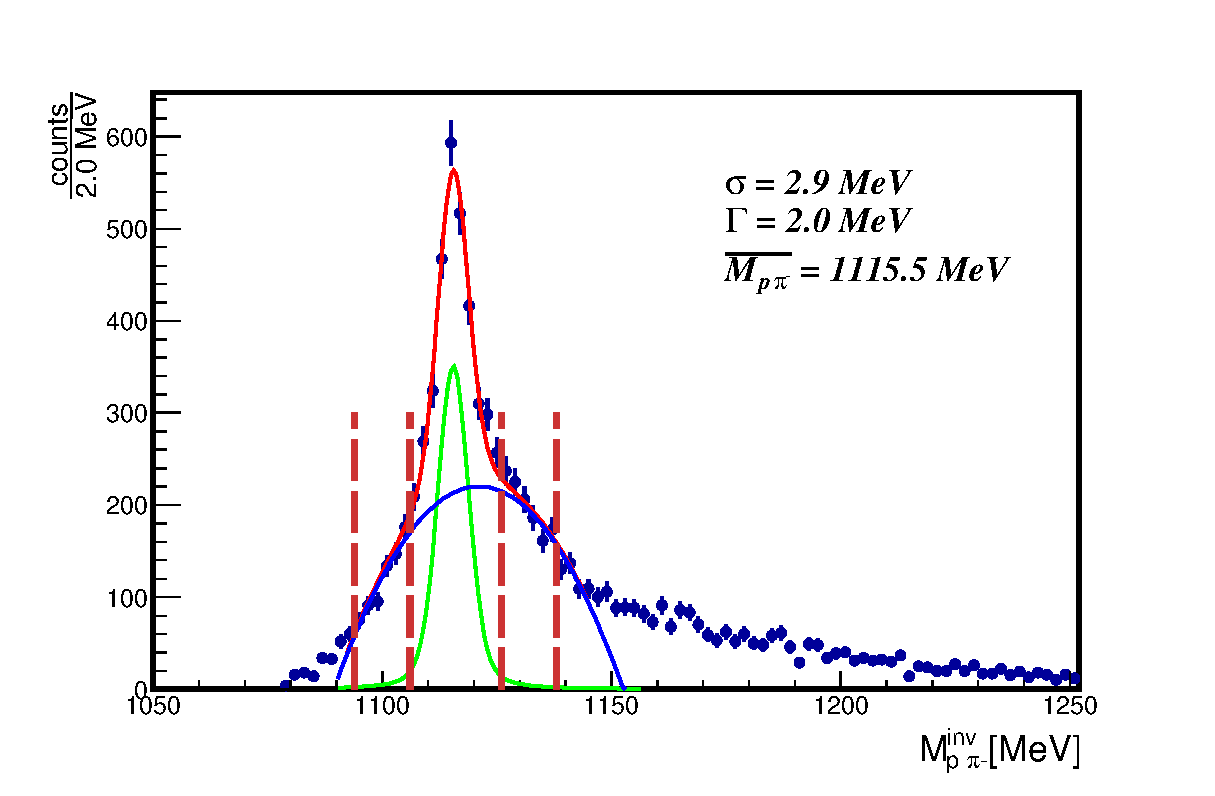
\includegraphics[width=0.7 \linewidth]{Chapter_analysisPNb/Lz.eps}
  \caption{The $\Lz$ spectrum after a neural network analysis obtained for pNb experiment. Color coding the same as in fig. \ref{fig:L1116SB}, vertical lines denotes regions of a side-band and are adjusted for pNb data.}
  \label{fig:L1116SB_pNb}
\end{figure}

\section{The $\Lz \Kz $reconstruction}
\begin{figure}[ht]
  \centering
  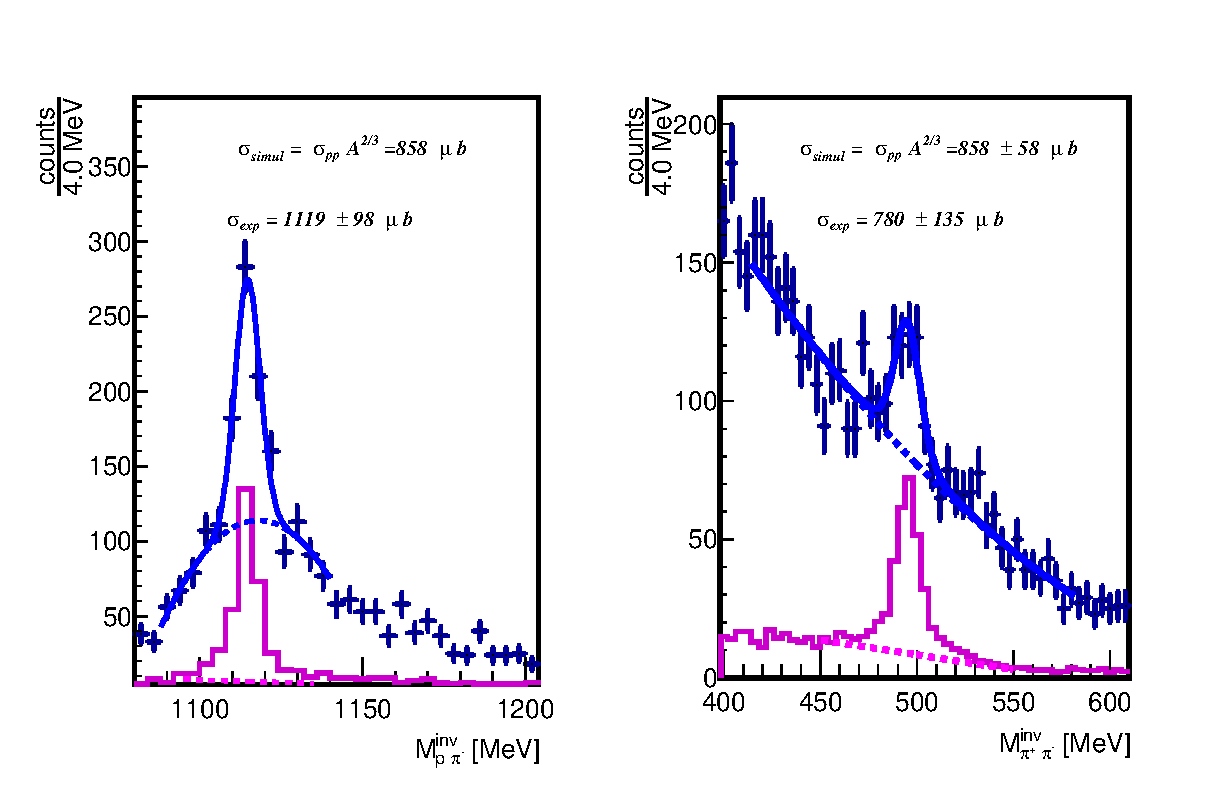
\includegraphics[width=0.9 \linewidth]{Chapter_analysisPNb/LK0.eps}
  \caption{The inclusive $\Lz \Kz$ spectrum obtained for pNb experiment. The \css for the simulation was scaled up by a factor $A^{2/3}$ compare values measured in pp reactions}
  \label{fig:LK0_pNb}
\end{figure}

\section{The $\Ls$ Reconstruction}



\subsection{Event mixing}


\subsection{Cross-section and extraction differential analysis}
\begin{figure}[ht]
  \centering
  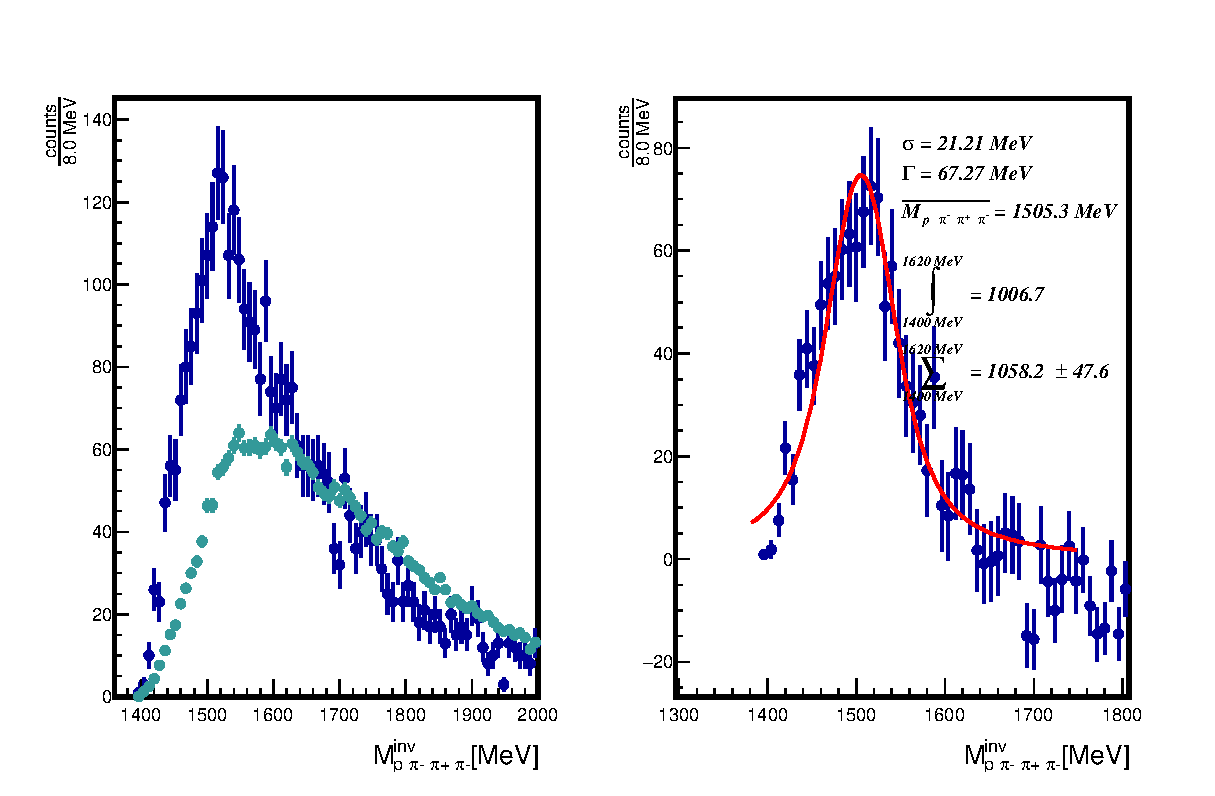
\includegraphics[width=0.9 \linewidth]{Chapter_analysisPNb/L1520.eps}
  \caption{a}
  \label{fig:L1520_pNb}
\end{figure}

\begin{figure}[ht]
  \centering
  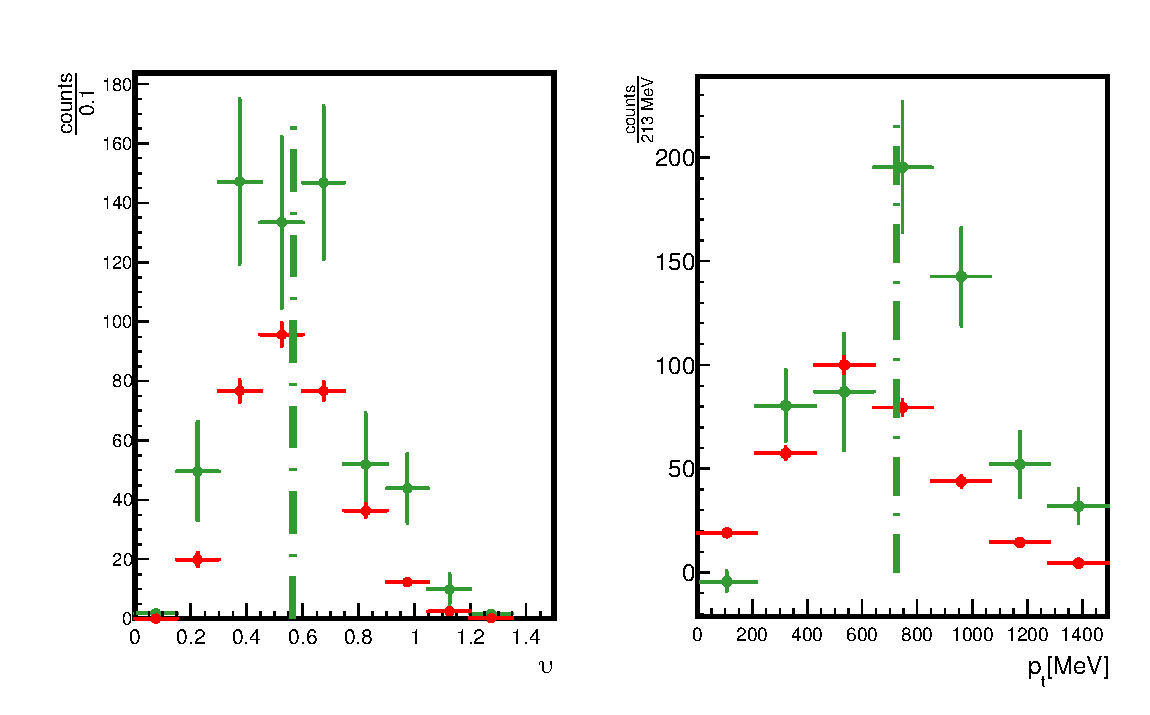
\includegraphics[width=0.9 \linewidth]{Chapter_analysisPNb/YPt.eps}
  \caption{b}
  \label{fig:YPt_pNb}
\end{figure}

\subsection{Analysis of a $\pip \pim$ spectrum}

\section{Comparison with results from pp data}